% Maybe this should move to progress section
\section{Medical Segmentation}
\subsection{Unet \& Friends}
This section we introduce several well known methods in medical segmentation. Unet \cite{ronneberger_u-net_2015} and its variations plays a dominant role in current medical segmentation tasks, and it is often used as a baseline model for performance evaluation in the literature.\\

Unet \cite{ronneberger_u-net_2015} is among one of the most widely used medical segmentation models since the day it was proposed. The original Unet consists of a contracting path followed by an expansive path that gives a "U" shaped architecture. The network architecture is shown in figure \ref{fig:unet-arch}.
Later this 2D model was extended to 3D version in \cite{ourselin_3d_2016} for for Kidney segmentation tasks so that the model learn features from information implicated between slices.\\
\begin{figure}
\centering
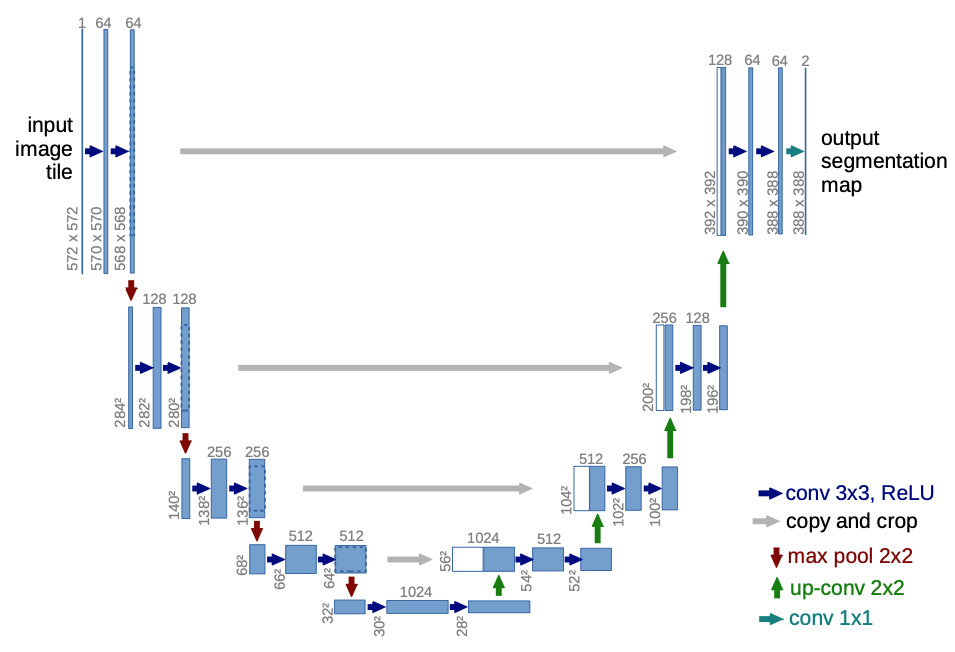
\includegraphics[width = 0.8\textwidth]{img/Unet_architecture}
\caption{Original Unet architecture in \cite{ronneberger_u-net_2015}}
\label{fig:unet-arch}
\end{figure}

VNet \cite{milletari_v-net_2016} is another 3D variation of Unet, and the network performed evaluation on prostate dataset. Each block of convolution has a residual feature that the input of the block is added to the last convolutional layer. The author argued that leverage residual structure enables network convergence in a fraction of the amount of time other network used.
%TODO insert residual structure here
\subsection{Loss functions for medical segmentation}
% TODO Loss/objectives here
Loss function or objective function is a crutial component in neural network training. Segmentation tasks usually make use of \textit{Distribution loss}, \textit{Region based loss} and \textit{boundary-based} loss for training and evaluation of segmentation performance.\\

Cross entropy (CE) measures the dissimilarity between the learned distribution and target distribution. Unet \cite{ronneberger_u-net_2015} training extend the CE by adding weight measured by, for example, inverse proportion of observed class frequency. This modification potentially deal with imbalance class which is very common in medical domain.\\

Dice loss is a region based loss function that learn to optimize the Dice Coefficient. Dice loss usually require the label to be one hot encoded during training. One benefit is that Dice loss does not requires class balance methods such as weighting method in CE loss.\\

Boundary loss aims to minimize the bourdary distance between prediction and ground-truth segmentation masks. Similar to Dice loss, it also alleviate the class imbalance issue during training.